\addcontentsline{toc}{chapter}{Занятие 15. Цепи Маркова. Период состояний.
                                Инвариантное распределение.}
\chapter*{Занятие 15. Цепи Маркова. Период состояний. Инвариантное распределение.}

\addcontentsline{toc}{section}{Контрольные вопросы и задания}
\section*{Контрольные вопросы и задания}

\subsubsection*{Приведите определение цепи Маркова.}

Последовательность дискретных случайных величин $ \left\{ x_n \right\}_{n \geq 0}$
называется простой цепью Маркова (с дискретным временем), если
\begin{equation*}
  P \left( x_{n + 1} = i_{n + 1} \; \middle| \; x_n = i_n, \dotsc, x_0 = i_0 \right) =
  P \left( x_{n + 1} = i_{n + 1} \; \middle| \; x_n = i_n \right).
\end{equation*}

\subsubsection*{Что называется переходными вероятностями цепи Маркова?}

Матрица $P \left( n \right) $,
где $P_{ij} \left( n \right) = P \left( x_{n + 1} = i_{n + 1} \; \middle| \; x_n = i \right) $,
называется матрицей переходных вероятностей на $n$-м шаге.

\subsubsection*{Как вычисляются переходные вероятности цепи Маркова за $n$ шагов?}

Матрица переходных вероятностей за $n$ шагов однородной цепи Маркова есть $n$-я
степень матрицы переходных вероятностей за 1 шаг.

\subsubsection*{Запишите уравнение Колмогорова-Чепмена.}

$P \left( x_n - i_n \; \middle| \; x_0 = i_0 \right) =
  \left( P^n \right)_{i_0, i_n}$.

\subsubsection*{Опишите, как классифицируются состояния цепи Маркова.}

Группы состояний марковской цепи (подмножества вершин графа переходов),
которым соответствуют тупиковые вершины диаграммы порядка графа переходов,
называются эргодическими классами цепи.
Состояния, которые находятся в эргодических классах, называются существенными,
а остальные~---~несущественными.
Поглощающее состояние является частным случаем эргодического класса.
Тогда попав в такое состояние, процесс прекратится.

\subsubsection*{Что называется периодом состояния?}

Пусть дана однородная цепь Маркова с дискретным временем $ \left\{ x_n \right\}_{n \geq 0}$
с матрицей переходных вероятностей $P$.
В частности, для любого $n \in \mathbb{N}$,
матрица $P^n = \left( p_{ij}^{ \left( n \right) } \right) $
является матрицей переходных вероятностей за $n$ шагов.
Рассмотрим последовательность $p_{jj}^{ \left( n \right) }, \, n \in \mathbb{N}$.
Число
\begin{equation*}
  d \left( j \right) =
  gcd \left( n \in \mathbb{N} \; \middle| \; p_{jj}^{ \left( n \right) } > 0 \right),
\end{equation*}
где $gcd$ обозначает наибольший общий делитель, называется периодом состояния $j$.

\subsubsection*{Сформулируйте утверждение про периоды сообщающихся состояний.}

Периоды сообщающихся состояний совпадают:
$ \left( i \leftrightarrow j \right) \Rightarrow \left( d \left( i \right) =
  d \left( j \right) \right) $.

\subsubsection*{Сформулируйте теорему про ассимптотическое поведение переходных вероятностей
                $p_{ij}^{ \left( n \right) }$ при $n \to \infty $.}

При $n \to \infty $ матрица $P^n$ стремится к строго положительной матрице,
у которой все строки совпадают с равновесным распределением.

\subsubsection*{Дайте определение инвариантного распределения цепи Маркова.}

Будем предполагать,
что $ \sigma $-алгебра $ \varepsilon $ порождена счётным семейством подмножеств $E$.

Всякая $ \sigma $-конечная мера $ \pi \left( \cdot \right) $, удовлетворяющая уравнению
\begin{equation*}
  \pi \left( A \right) = \int \limits_{E} \pi \left( dx \right) P \left( x, A \right), \,
  A \in \varepsilon
\end{equation*}
и условию $ \pi \left( A \right) < \infty $ хотя бы для одного множества $A \in \varepsilon^+$,
называется инвариантной.

\addcontentsline{toc}{section}{Аудиторные задачи}
\section*{Аудиторные задачи}

\subsubsection*{15.4}

\textit{Задание.}
По виду матрицы переходных вероятностей проведите классификацию состояний соответствующей цепи
Маркова и найдите её инвариантное распределение.
\begin{enumerate}[label=\alph*)]
  \item \begin{equation*}
    P =
    \begin{bmatrix}
      0 & 0 & \frac{1}{3} & \frac{1}{3} & \frac{1}{3} \\
      0 & \frac{1}{3} & \frac{1}{3} & \frac{1}{3} & 0 \\
      \frac{1}{4} & \frac{1}{4} & \frac{1}{4} & \frac{1}{4} & 0 \\
      0 & 0 & 0 & \frac{1}{2} & \frac{1}{2} \\
      0 & 0 & 0 & \frac{1}{2} & \frac{1}{2}
    \end{bmatrix};
  \end{equation*}
  \item \begin{equation*}
      P =
      \begin{bmatrix}
        0 & 0 & 0 & \frac{1}{2} & \frac{1}{2} \\
        0 & \frac{1}{2} & \frac{1}{2} & 0 & 0 \\
        0 & 1 & 0 & 0 & 0 \\
        0 & 1 & 0 & 0 & 0 \\
        0 & 0 & 0 & 1 & 0
      \end{bmatrix}.
  \end{equation*}
\end{enumerate}

\textit{Решение.}
\begin{enumerate}[label=\alph*)]
  \item $ \pi = \left( \pi_1, \pi_2, \pi_3, \pi_4, \pi_5 \right) $.

  Инвариантное распределение можно найти из условия $ \pi P = \pi $.

  Получим систему уравнений
  \begin{equation*}
    \begin{cases}
      \frac{ \pi_3}{4} = \pi_1, \\
      \frac{ \pi_2}{3} + \frac{ \pi_3}{4} = \pi_2, \\
      \frac{ \pi_1}{3} + \frac{ \pi_2}{3} + \frac{ \pi_3}{4} = \pi_3, \\
      \frac{ \pi_1}{3} + \frac{ \pi_2}{3} + \frac{ \pi_3}{4} + \frac{ \pi_4}{2} + \frac{ \pi_2}{5} =
      \pi_4, \\
      \frac{ \pi_1}{3} + \frac{ \pi_4}{2} + \frac{ \pi_5}{2} = \pi_5, \\
      \pi_1 + \pi_2 + \pi_3 + \pi_4 + \pi_5 = 1,
    \end{cases}
  \end{equation*}
  где последнее уравнение возникло из-за того, что это распределение.

  Это система однородных уравнений.

  Решений не больше одного.
  Теперь найдём это решение.

  $ \pi_3 = 4 \pi_1$.
  Подставим это во второе уравнение
  \begin{equation*}
    \frac{ \pi_2}{3} + \pi_1 = \pi_2 \Rightarrow
    \frac{2 \pi_2}{3} = \pi_1 \Rightarrow
    \pi_2 = \frac{3 \pi_1}{2}.
  \end{equation*}

  Получим уравнение для нахождения $ \pi_1$, то есть
  \begin{equation*}
    \frac{ \pi_1}{3} + \frac{ \pi_1}{2} + \pi_1 =
    4 \pi_1.
  \end{equation*}

  Приведём подобные
  \begin{equation*}
    \frac{5 \pi_1}{6} = 3 \pi_1 \Rightarrow \pi_1 = 0.
  \end{equation*}

  Отсюда следует, что $ \pi_2 = 0, \, \pi_3 = 0$.

  Остаётся 2 уравнения
  \begin{equation*}
    \begin{cases}
      \frac{ \pi_4}{2} + \frac{ \pi_5}{2} = \pi_4 \Rightarrow \pi_4 = \pi_5, \\
      \pi_4 + \pi_5 = 1.
    \end{cases}
  \end{equation*}

  Отсюда
  \begin{equation*}
    \pi_4 =
    \pi_5 =
    \frac{1}{2}.
  \end{equation*}

  Ответ: инвариантное распределение
  \begin{equation*}
    \left( 0, 0, 0, \frac{1}{2}, \frac{1}{2} \right).
  \end{equation*}
  Почему так получается?
  Посмотрим, какие есть переходы в этой цепи.
  Есть 5 состояний (рис. \ref{fig:154}).

  \begin{figure}[h!]
    \centering
    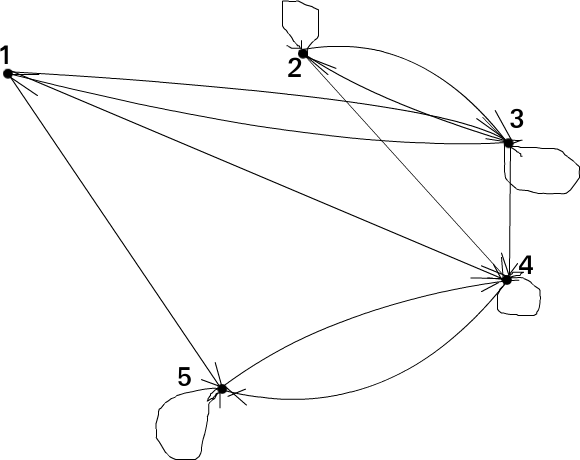
\includegraphics[width=.4\textwidth]{./pictures/15_4.png}
    \caption{Состояния и переходы цепи Маркова}
    \label{fig:154}
  \end{figure}

  $4 \leftrightarrow 5$~---~существенные.

  $1 \leftrightarrow 2 \leftrightarrow 3$~---~несущественные.

  Инвариантное распределение не может иметь положительную вероятность на несущественном состоянии.
  \item Найдём инвариантное распределение для такой матрицы (рис. \ref{fig:1541}).

  \begin{figure}[h!]
    \centering
    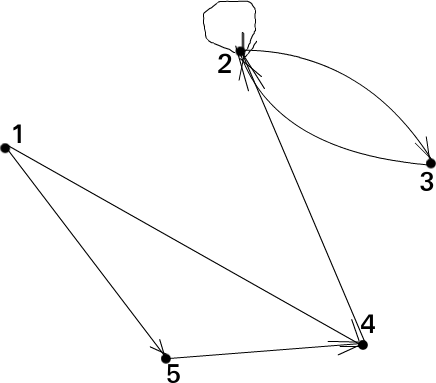
\includegraphics[width=.4\textwidth]{./pictures/15_4_1.png}
    \caption{Состояния и переходы цепи Маркова}
    \label{fig:1541}
  \end{figure}

$2 \leftrightarrow 3$.

Состояния $1, 4, 5$~---~несущественные.

Это значит, что
\begin{equation*}
  \pi \; : \;
  \left( 0, \frac{1}{3}, \frac{2}{3}, 0, 0 \right).
\end{equation*}

Только 2 состояния существенные, значит, уравнения будут такими:
\begin{equation*}
  \begin{cases}
    \frac{ \pi_2}{2} + \pi_3 = \pi_2, \\
    \frac{ \pi_2}{2} = \pi_3, \\
    \pi_2 + \pi_3 = 1.
  \end{cases}
\end{equation*}
\end{enumerate}

\subsubsection*{15.5}

\textit{Задание.}
Найдите инвариантное распределение симметрического блуждания на $ \left[ 0, N \right] $
с поглощением на концах.

\textit{Решение.}
$ \left\{ X_n \right\}_{n \geq 0}$~---~это симметричное случайное блуждание с поглощением в точках
$ \left\{ 0, N \right\} $.
Представим себе, как такая цепь движется.
Цепь принимает значения в отрезке (рис. \ref{fig:155}).

\begin{figure}[h!]
  \centering
  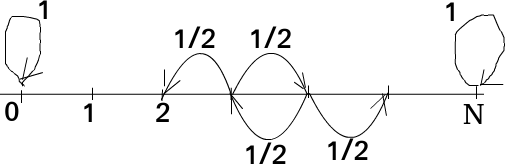
\includegraphics[width=.4\textwidth]{./pictures/15_5.png}
  \caption{Состояния и переходы цепи Маркова}
  \label{fig:155}
\end{figure}

Напишем матрицу переходных вероятностей
\begin{equation*}
  P =
  \begin{bmatrix}
    1 & 0 & 0 & 0 & \dotsc & 0 \\
    \frac{1}{2} & 0 & \frac{1}{2} & 0 & \dotsc & 0 \\
    \dotsc & \dotsc & \dotsc & \dotsc & \dotsc & \dotsc & \\
    0 & 0 & 0 & 0 & \dotsc & 1
  \end{bmatrix}.
\end{equation*}

Как тут будет выглядеть инвариантное распределение?

Все состояния кроме концов отрезка несущественные.
Это означает, что $ \pi_i = 0, \, i \neq 0, N$.

Получаем систему уравненеий
\begin{equation*}
  \begin{cases}
    \pi_1 = \pi_1, \\
    \pi_N = \pi_N, \\
    \pi_1 + \pi_N = 1.
  \end{cases}
\end{equation*}

Это означает, что у нас только одно уравнение на эти вероятности.

Тут инвариантных распределений бесконечно много.
Любое инвариантное распределение имеет вид $ \left( \pi_1, 0, 0, 0, \dotsc, 0, 1 - \pi_1 \right) $.

\addcontentsline{toc}{section}{Домашнее задание}
\section*{Домашнее задание}

\subsubsection*{15.12}

\textit{Задание.}
По виду матрицы переходных вероятностей проведите классификацию состояний соответственной цепи
Маркова и найдите его инвариантное распределение.
\begin{equation*}
  P =
  \begin{bmatrix}
    \frac{1}{2} & 0 & \frac{1}{2} & 0 & 0 \\
    0 & \frac{1}{2} & 0 & 0 & \frac{1}{2} \\
    0 & 0 & 0 & 1 & 0 \\
    \frac{1}{3} & 0 & \frac{1}{3} & \frac{1}{3} & 0 \\
    \frac{1}{2} & 0 & 0 & 0 & \frac{1}{2}
  \end{bmatrix}.
\end{equation*}

\textit{Решение.}
$ \pi = \left( \pi_1, \pi_2, \pi_3, \pi_4, \pi_5 \right) $.

Инвариантное распределение можно найти из условия $ \pi P = \pi $.

Получим систему уравнений
\begin{equation*}
  \begin{cases}
    \frac{ \pi_1}{2} + \frac{ \pi_4}{3} + \frac{ \pi_5}{2} = \pi_1, \\
    \frac{ \pi_2}{2} = \pi_2, \\
    \frac{ \pi_1}{2} + \frac{ \pi_4}{3} = \pi_3, \\
    \pi_3 + \frac{ \pi_4}{3} = \pi_4, \\
    \frac{ \pi_2}{2} + \frac{ \pi_5}{2} = \pi_5, \\
    \pi_1 + \pi_2 + \pi_3 + \pi_4 + \pi_5 = 1,
  \end{cases}
\end{equation*}
где последнее уравнение возникло из-за того, что это распределение.

Это система однородных уравнений.

Решений не больше одного.
Теперь найдём это решение.

$ \pi_2 = 0$.
Подставим это в пятое уравнение
\begin{equation*}
  \frac{ \pi_5}{2} = \pi_5, \Rightarrow
  \pi_5 = 0.
\end{equation*}

Остаются уравнения
\begin{equation*}
  \begin{cases}
    \frac{ \pi_1}{2} + \frac{ \pi_4}{3} = \pi_1, \\
    \frac{ \pi_1}{2} + \frac{ \pi_4}{3} = \pi_3, \\
    \pi_3 + \frac{\pi_4}{3} = \pi_4, \\
    \pi_1 + \pi_3 + \pi_4 = 1.
  \end{cases}
\end{equation*}

Из первого уравнения получаем
\begin{equation*}
  \frac{ \pi_4}{3} = \pi_1 - \frac{ \pi_1}{2} = \frac{ \pi_1}{2} \Rightarrow
  \pi_4 = \frac{3 \pi_1}{2}.
\end{equation*}
Подставим во второе уравнение
\begin{equation*}
  \frac{ \pi_1}{2} + \frac{ \pi_1}{2} =
  \pi_3 = \pi_1.
\end{equation*}

Подставим в последонее уравнение
\begin{equation*}
  \pi_1 + \pi_1 + \frac{3 \pi_1}{2} = 1 \Rightarrow
  2 \pi_1 + \frac{3 \pi_1}{2} = 1 \Rightarrow
  \frac{7 \pi_1}{2} = 1 \Rightarrow
  \pi_1 = \frac{2}{7} \Rightarrow
  \pi_4 = \frac{3}{2} \cdot \frac{2}{7} = \frac{3}{7}.
\end{equation*}

Ответ: инвариантное распределение:
\begin{equation*}
  \left( \frac{2}{7}, 0, \frac{2}{7}, \frac{3}{7}, 0 \right).
\end{equation*}

Почему так получилось?
Посмотрим, какие есть переходы в этой цепи?

Есть 5 состояний (рис. \ref{fig:1512}).

\begin{figure}[h]
  \centering
  \includestandalone[mode=buildnew]{./pictures/15_12}
  \caption{Состояния и переходы цепи Маркова}
  \label{fig:1512}
\end{figure}

$1 \leftrightarrow 3 \leftrightarrow 4$~---~существенные.

$2, 5$~---~несущественные.

Инвариантное распределение не может иметь положительную вероятность на несущественном состоянии.

\subsubsection*{15.13}

\textit{Задание.}
Найдите инвариантное распределение симметрического блуждания на $ \left[ 0, N \right] $
\begin{enumerate}[label=\alph*)]
  \item с отражением на концах;
  \item с отражением на одном из концов и поглощением на другом.
\end{enumerate}

\textit{Решение.}
\begin{enumerate}[label=\alph*)]
  \item $ \left\{ X_n \right\} $~---~симметрическое блуждание с отражением в точках
  $ \left\{ 0, N \right\} $.

  Представим себе, как такая цепь движется.
  Цепь принимает значения в отрезке (рис. \ref{fig:1513}).

  \begin{figure}[h]
    \centering
    \includestandalone[mode=buildnew, width=.9\textwidth]{./pictures/15_13}
    \caption{Состояния и переходы цепи Маркова}
    \label{fig:1513}
  \end{figure}

  Напишем матрицу переходных вероятностей
  \begin{equation*}
    P =
    \begin{bmatrix}
      0 & 1 & 0 & 0 & \dotsc & 0 \\
      \frac{1}{2} & 0 & \frac{1}{2} & 0 & \dotsc & 0 \\
      0 & \frac{1}{2} & 0 & \frac{1}{2} & \dotsc & 0 \\
      \dotsc & \dotsc & \dotsc & \dotsc & \dotsc & \dotsc \\
      0 & 0 & 0 & 0 & \dotsc & 0
    \end{bmatrix}.
  \end{equation*}

  Как тут будет выглядеть инвариантное распределение?

  Получается система уравнений
  \begin{equation*}
    \begin{cases}
      \frac{1}{2} \cdot \pi_1 = \pi_0, \\
      \pi_0 + \frac{1}{2} \cdot \pi_2 = \pi_1, \\
      \frac{1}{2} \cdot \pi_1 + \frac{1}{2} \cdot \pi_3 = \pi_2, \\
      \frac{1}{2} \cdot \pi_2 + \frac{1}{2} \cdot \pi_4 = \pi_3, \\
      \dotsc, \\
      \frac{1}{2} \cdot \pi_{N - 1} = \pi_N, \\
      \pi_0 + \pi_1 + \dotsc + \pi_N = 1.
    \end{cases}
  \end{equation*}

  Из первого уравнения $ \pi_1 = 2 \pi_0$.

  Подставим это во второе уравнение
  \begin{equation*}
    \pi_0 + \frac{1}{2} \cdot \pi_2 = 2 \pi_0 \Rightarrow
    \pi_0 = \frac{1}{2} \cdot \pi_2 \Rightarrow
    \pi_2 = 2 \pi_0.
  \end{equation*}

  Подставим это в третье уравнение
  \begin{equation*}
    \pi_0 + \frac{1}{2} \cdot \pi_3 = 2 \pi_0 \Rightarrow
    \pi_0 = \frac{1}{2} \cdot \pi_3 \Rightarrow
    \pi_3 = 2 \pi_0.
  \end{equation*}

  Таким образом, $ \pi_1 = \pi_2 = \dotsc = \pi_{N - 1} = 2 \pi_0, \, \pi_N = \pi_0$.

  Подставим это в последнее уравнение $ \pi_0 + 2 \pi_0 \left( N - 1 \right) + \pi_0 = 1$.

  Приведём подобные
  \begin{equation*}
    N \pi_0 = \frac{1}{2}.
  \end{equation*}

  Отсюда находим, что
  \begin{equation*}
    \pi_0 =
    \frac{1}{2N} =
    \pi_N.
  \end{equation*}

  Значит,
  \begin{equation*}
    \pi_1 =
    \dotsc =
    \pi_{N - 1} =
    \frac{1}{N}.
  \end{equation*}

  Инвариантное распределение имеет вид
  \begin{equation*}
    \left( \frac{1}{2N}, \frac{1}{N}, \dotsc, \frac{1}{N}, \frac{1}{2N} \right);
  \end{equation*}
  \item последовательность случайных величин
  $ \left\{ X_n \right\}_{n \geq 0}$~---~симметричное случайное блуждание с поглощением в точке
  $ \left\{ 0 \right\} $ и отражением в точке $ \left\{ N \right\} $.
  Представим себе, как такая цепь движется.
  Цепь принимает значения на отрезке (рис. \ref{fig:15131}).

  \begin{figure}[h]
    \centering
    \includestandalone[mode=buildnew, width=.9\textwidth]{./pictures/15_13_1}
    \caption{Состояния и переходы цепи Маркова}
    \label{fig:15131}
  \end{figure}

  Напишем матрицу переходных вероятностей
  \begin{equation*}
    P =
    \begin{bmatrix}
      1 & 0 & 0 & 0 & \dotsc & 0 \\
      \frac{1}{2} & 0 & \frac{1}{2} & 0 & \dotsc & 0 \\
      \dotsc & \dotsc & \dotsc & \dotsc & \dotsc & \dotsc \\
      0 & 0 & 0 & 0 & \dotsc & 0
    \end{bmatrix}.
  \end{equation*}

  Как тут будет выглядеть инвариантное распределение?

  Все состояния кроме $ \left\{ 0 \right\} $ несущественные.
  Это означает, что
  \begin{equation*}
    \pi_i = 0, \,
    i \neq 0.
  \end{equation*}

  Получаем систему уравнений
  \begin{equation*}
    \begin{cases}
      \pi_1 = \pi_1, \\
      \pi_1 = 1.
  \end{cases}
  \end{equation*}

  Тут инвариантное распределение имеет вид $ \left( 1, 0, 0, 0, \dotsc, 0, 0 \right) $.
\end{enumerate}
